% Options for packages loaded elsewhere
\PassOptionsToPackage{unicode}{hyperref}
\PassOptionsToPackage{hyphens}{url}
%
\documentclass[
  ignorenonframetext,
]{beamer}
\usepackage{pgfpages}
\setbeamertemplate{caption}[numbered]
\setbeamertemplate{caption label separator}{: }
\setbeamercolor{caption name}{fg=normal text.fg}
\beamertemplatenavigationsymbolsempty
% Prevent slide breaks in the middle of a paragraph
\widowpenalties 1 10000
\raggedbottom
\setbeamertemplate{part page}{
  \centering
  \begin{beamercolorbox}[sep=16pt,center]{part title}
    \usebeamerfont{part title}\insertpart\par
  \end{beamercolorbox}
}
\setbeamertemplate{section page}{
  \centering
  \begin{beamercolorbox}[sep=12pt,center]{part title}
    \usebeamerfont{section title}\insertsection\par
  \end{beamercolorbox}
}
\setbeamertemplate{subsection page}{
  \centering
  \begin{beamercolorbox}[sep=8pt,center]{part title}
    \usebeamerfont{subsection title}\insertsubsection\par
  \end{beamercolorbox}
}
\AtBeginPart{
  \frame{\partpage}
}
\AtBeginSection{
  \ifbibliography
  \else
    \frame{\sectionpage}
  \fi
}
\AtBeginSubsection{
  \frame{\subsectionpage}
}

\usepackage{amsmath,amssymb}
\usepackage{iftex}
\ifPDFTeX
  \usepackage[T1]{fontenc}
  \usepackage[utf8]{inputenc}
  \usepackage{textcomp} % provide euro and other symbols
\else % if luatex or xetex
  \usepackage{unicode-math}
  \defaultfontfeatures{Scale=MatchLowercase}
  \defaultfontfeatures[\rmfamily]{Ligatures=TeX,Scale=1}
\fi
\usepackage{lmodern}
\usetheme[]{Boadilla}
\usecolortheme{rose}
\ifPDFTeX\else  
    % xetex/luatex font selection
\fi
% Use upquote if available, for straight quotes in verbatim environments
\IfFileExists{upquote.sty}{\usepackage{upquote}}{}
\IfFileExists{microtype.sty}{% use microtype if available
  \usepackage[]{microtype}
  \UseMicrotypeSet[protrusion]{basicmath} % disable protrusion for tt fonts
}{}
\makeatletter
\@ifundefined{KOMAClassName}{% if non-KOMA class
  \IfFileExists{parskip.sty}{%
    \usepackage{parskip}
  }{% else
    \setlength{\parindent}{0pt}
    \setlength{\parskip}{6pt plus 2pt minus 1pt}}
}{% if KOMA class
  \KOMAoptions{parskip=half}}
\makeatother
\usepackage{xcolor}
\newif\ifbibliography
\setlength{\emergencystretch}{3em} % prevent overfull lines
\setcounter{secnumdepth}{-\maxdimen} % remove section numbering

\usepackage{color}
\usepackage{fancyvrb}
\newcommand{\VerbBar}{|}
\newcommand{\VERB}{\Verb[commandchars=\\\{\}]}
\DefineVerbatimEnvironment{Highlighting}{Verbatim}{commandchars=\\\{\}}
% Add ',fontsize=\small' for more characters per line
\usepackage{framed}
\definecolor{shadecolor}{RGB}{241,243,245}
\newenvironment{Shaded}{\begin{snugshade}}{\end{snugshade}}
\newcommand{\AlertTok}[1]{\textcolor[rgb]{0.68,0.00,0.00}{#1}}
\newcommand{\AnnotationTok}[1]{\textcolor[rgb]{0.37,0.37,0.37}{#1}}
\newcommand{\AttributeTok}[1]{\textcolor[rgb]{0.40,0.45,0.13}{#1}}
\newcommand{\BaseNTok}[1]{\textcolor[rgb]{0.68,0.00,0.00}{#1}}
\newcommand{\BuiltInTok}[1]{\textcolor[rgb]{0.00,0.23,0.31}{#1}}
\newcommand{\CharTok}[1]{\textcolor[rgb]{0.13,0.47,0.30}{#1}}
\newcommand{\CommentTok}[1]{\textcolor[rgb]{0.37,0.37,0.37}{#1}}
\newcommand{\CommentVarTok}[1]{\textcolor[rgb]{0.37,0.37,0.37}{\textit{#1}}}
\newcommand{\ConstantTok}[1]{\textcolor[rgb]{0.56,0.35,0.01}{#1}}
\newcommand{\ControlFlowTok}[1]{\textcolor[rgb]{0.00,0.23,0.31}{#1}}
\newcommand{\DataTypeTok}[1]{\textcolor[rgb]{0.68,0.00,0.00}{#1}}
\newcommand{\DecValTok}[1]{\textcolor[rgb]{0.68,0.00,0.00}{#1}}
\newcommand{\DocumentationTok}[1]{\textcolor[rgb]{0.37,0.37,0.37}{\textit{#1}}}
\newcommand{\ErrorTok}[1]{\textcolor[rgb]{0.68,0.00,0.00}{#1}}
\newcommand{\ExtensionTok}[1]{\textcolor[rgb]{0.00,0.23,0.31}{#1}}
\newcommand{\FloatTok}[1]{\textcolor[rgb]{0.68,0.00,0.00}{#1}}
\newcommand{\FunctionTok}[1]{\textcolor[rgb]{0.28,0.35,0.67}{#1}}
\newcommand{\ImportTok}[1]{\textcolor[rgb]{0.00,0.46,0.62}{#1}}
\newcommand{\InformationTok}[1]{\textcolor[rgb]{0.37,0.37,0.37}{#1}}
\newcommand{\KeywordTok}[1]{\textcolor[rgb]{0.00,0.23,0.31}{#1}}
\newcommand{\NormalTok}[1]{\textcolor[rgb]{0.00,0.23,0.31}{#1}}
\newcommand{\OperatorTok}[1]{\textcolor[rgb]{0.37,0.37,0.37}{#1}}
\newcommand{\OtherTok}[1]{\textcolor[rgb]{0.00,0.23,0.31}{#1}}
\newcommand{\PreprocessorTok}[1]{\textcolor[rgb]{0.68,0.00,0.00}{#1}}
\newcommand{\RegionMarkerTok}[1]{\textcolor[rgb]{0.00,0.23,0.31}{#1}}
\newcommand{\SpecialCharTok}[1]{\textcolor[rgb]{0.37,0.37,0.37}{#1}}
\newcommand{\SpecialStringTok}[1]{\textcolor[rgb]{0.13,0.47,0.30}{#1}}
\newcommand{\StringTok}[1]{\textcolor[rgb]{0.13,0.47,0.30}{#1}}
\newcommand{\VariableTok}[1]{\textcolor[rgb]{0.07,0.07,0.07}{#1}}
\newcommand{\VerbatimStringTok}[1]{\textcolor[rgb]{0.13,0.47,0.30}{#1}}
\newcommand{\WarningTok}[1]{\textcolor[rgb]{0.37,0.37,0.37}{\textit{#1}}}

\providecommand{\tightlist}{%
  \setlength{\itemsep}{0pt}\setlength{\parskip}{0pt}}\usepackage{longtable,booktabs,array}
\usepackage{calc} % for calculating minipage widths
\usepackage{caption}
% Make caption package work with longtable
\makeatletter
\def\fnum@table{\tablename~\thetable}
\makeatother
\usepackage{graphicx}
\makeatletter
\def\maxwidth{\ifdim\Gin@nat@width>\linewidth\linewidth\else\Gin@nat@width\fi}
\def\maxheight{\ifdim\Gin@nat@height>\textheight\textheight\else\Gin@nat@height\fi}
\makeatother
% Scale images if necessary, so that they will not overflow the page
% margins by default, and it is still possible to overwrite the defaults
% using explicit options in \includegraphics[width, height, ...]{}
\setkeys{Gin}{width=\maxwidth,height=\maxheight,keepaspectratio}
% Set default figure placement to htbp
\makeatletter
\def\fps@figure{htbp}
\makeatother

\makeatletter
\makeatother
\makeatletter
\makeatother
\makeatletter
\@ifpackageloaded{caption}{}{\usepackage{caption}}
\AtBeginDocument{%
\ifdefined\contentsname
  \renewcommand*\contentsname{Table of contents}
\else
  \newcommand\contentsname{Table of contents}
\fi
\ifdefined\listfigurename
  \renewcommand*\listfigurename{List of Figures}
\else
  \newcommand\listfigurename{List of Figures}
\fi
\ifdefined\listtablename
  \renewcommand*\listtablename{List of Tables}
\else
  \newcommand\listtablename{List of Tables}
\fi
\ifdefined\figurename
  \renewcommand*\figurename{Figure}
\else
  \newcommand\figurename{Figure}
\fi
\ifdefined\tablename
  \renewcommand*\tablename{Table}
\else
  \newcommand\tablename{Table}
\fi
}
\@ifpackageloaded{float}{}{\usepackage{float}}
\floatstyle{ruled}
\@ifundefined{c@chapter}{\newfloat{codelisting}{h}{lop}}{\newfloat{codelisting}{h}{lop}[chapter]}
\floatname{codelisting}{Listing}
\newcommand*\listoflistings{\listof{codelisting}{List of Listings}}
\makeatother
\makeatletter
\@ifpackageloaded{caption}{}{\usepackage{caption}}
\@ifpackageloaded{subcaption}{}{\usepackage{subcaption}}
\makeatother
\makeatletter
\@ifpackageloaded{tcolorbox}{}{\usepackage[skins,breakable]{tcolorbox}}
\makeatother
\makeatletter
\@ifundefined{shadecolor}{\definecolor{shadecolor}{rgb}{.97, .97, .97}}
\makeatother
\makeatletter
\makeatother
\makeatletter
\makeatother
\ifLuaTeX
  \usepackage{selnolig}  % disable illegal ligatures
\fi
\IfFileExists{bookmark.sty}{\usepackage{bookmark}}{\usepackage{hyperref}}
\IfFileExists{xurl.sty}{\usepackage{xurl}}{} % add URL line breaks if available
\urlstyle{same} % disable monospaced font for URLs
\hypersetup{
  pdftitle={Recursion},
  pdfauthor={Salaar Liaqat},
  hidelinks,
  pdfcreator={LaTeX via pandoc}}

\title{Recursion}
\author{Salaar Liaqat}
\date{}
\institute{Data Sciences Institute, UofT}

\begin{document}
\frame{\titlepage}
\ifdefined\Shaded\renewenvironment{Shaded}{\begin{tcolorbox}[frame hidden, interior hidden, sharp corners, boxrule=0pt, breakable, borderline west={3pt}{0pt}{shadecolor}, enhanced]}{\end{tcolorbox}}\fi

\begin{frame}{Outline}
\protect\hypertarget{outline}{}
\begin{itemize}
\item
  Call Stack
\item
  Recursion
\item
  Time and Space complexity of Recursion
\item
  Mergesort
\item
  Multiple recursive
\end{itemize}
\end{frame}

\hypertarget{call-stack}{%
\section{Call Stack}\label{call-stack}}

\begin{frame}[fragile]{How a Call Stack Works}
\protect\hypertarget{how-a-call-stack-works}{}
\begin{itemize}
\item
  Your computer internally uses a call stack (stack ADT) to execute
  functions
\item
  When you run your Python file, the \texttt{main} functions is called.
  \texttt{main} is pushed onto the stack

  \begin{itemize}
  \tightlist
  \item
    Sounds familiar? \texttt{if\ \_\_name\_\_\ ==\ "\_\_main\_\_":}
  \end{itemize}
\item
  As the main function executes, it may call other functions, each
  functions is pushed to the top of the stack

  \begin{itemize}
  \tightlist
  \item
    The currently executing function is at the top of the stack
  \end{itemize}
\item
  When each function is executed, it is popped from the stack
\item
  The function may return a value, which is passes to the calling
  function (the function below in the stack).
\item
  The calling function can use the return value and continue execution
  until the stack is empty
\end{itemize}
\end{frame}

\begin{frame}[fragile]{Basic Example}
\protect\hypertarget{basic-example}{}
\begin{itemize}
\item
  If I run \texttt{round(float("20.24"))}, I expect \texttt{20}

  \begin{itemize}
  \item
    The \texttt{round} function is first to be called, it is pushed on
    the call stack
  \item
    Then, \texttt{float("20.24")} is called and pushed on the call stack
  \end{itemize}
\item
  Now, we pop each function off the call stack.

  \begin{itemize}
  \item
    \texttt{float("20.24")} returns \texttt{20.24}
  \item
    \texttt{round} uses the return value of the previous function,
    \texttt{20.24}. It executes \texttt{round(20.24)}, which returns
    \texttt{20}
  \item
    The stack is empty, so the program finishes
  \end{itemize}
\end{itemize}
\end{frame}

\hypertarget{recursion}{%
\section{Recursion}\label{recursion}}

\begin{frame}{Motivating Example}
\protect\hypertarget{motivating-example}{}
\begin{itemize}
\tightlist
\item
  Suppose you are looking for a key in a box, but the box contains more
  boxes!
\end{itemize}

\begin{figure}

{\centering 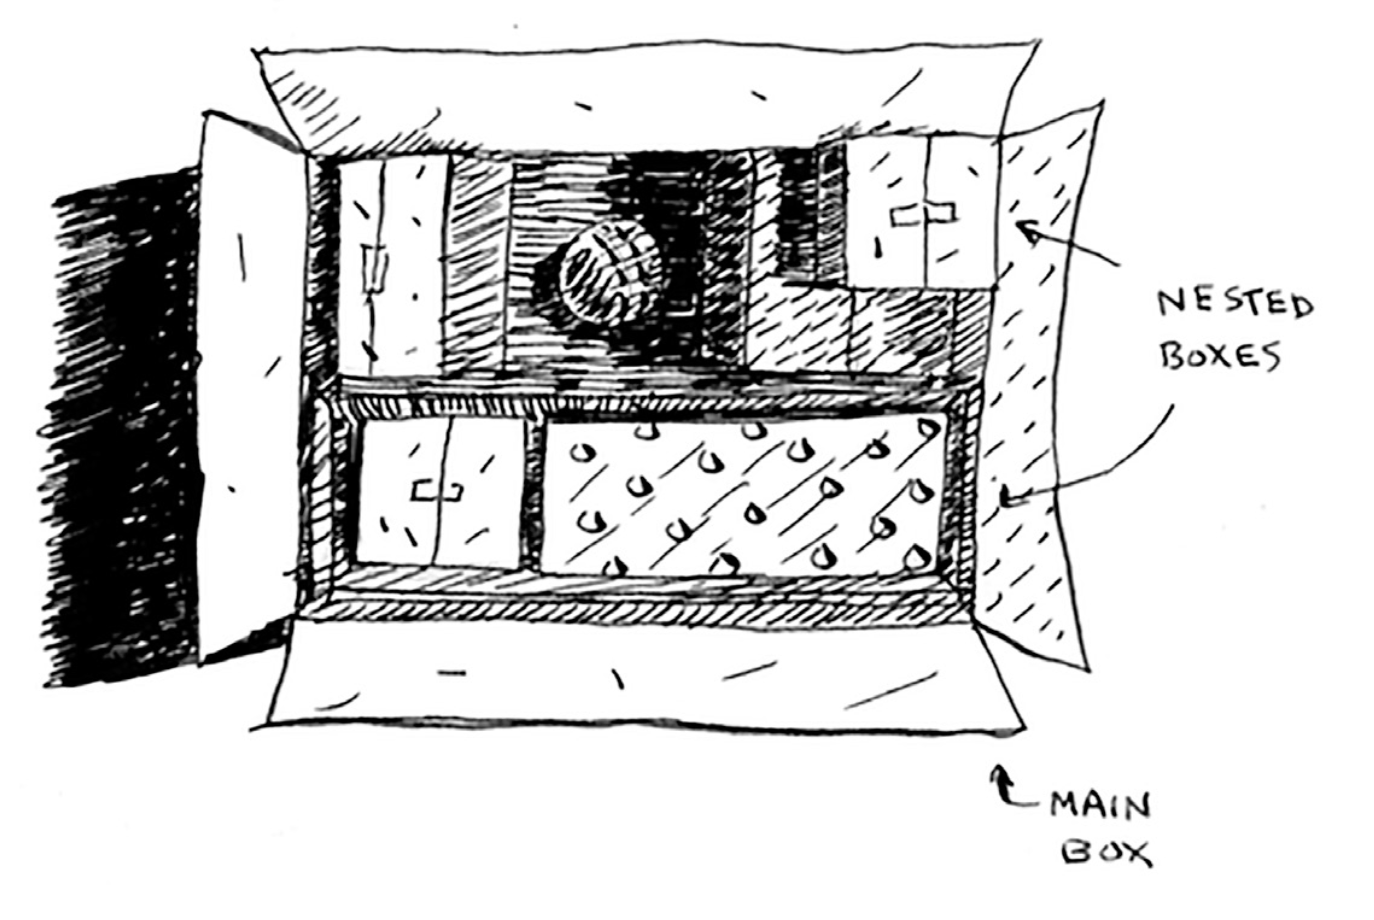
\includegraphics[width=7.9cm,height=\textheight]{images/box-recursion.png}

}

\end{figure}

\begin{itemize}
\tightlist
\item
  2 minutes: write down the steps of the algorithm you would take to
  search for the key
\end{itemize}
\end{frame}

\begin{frame}{Algorithm 1: Loop}
\protect\hypertarget{algorithm-1-loop}{}
\begin{enumerate}
\item
  Make a pile of all the boxes
\item
  Grab a box and open it
\item
  If it contains a box, append it to your pile of boxes
\item
  If it contains the key, you're done!
\item
  Repeat
\end{enumerate}
\end{frame}

\begin{frame}{Algorithm 2: Recursion}
\protect\hypertarget{algorithm-2-recursion}{}
\begin{enumerate}
\item
  Grab a box and open it
\item
  If it contains a box, repeat step 1
\item
  If it contains the key, you're done!
\end{enumerate}

\vspace{1cm}

\emph{Which algorithm do you like more?}

\begin{itemize}
\item
  Notice the function is recursive because it calls itself
\item
  Both algorithms achieve the same thing, but recursion is clearer (to
  me)
\end{itemize}
\end{frame}

\begin{frame}[fragile]{Formula to write a recursive function}
\protect\hypertarget{formula-to-write-a-recursive-function}{}
\begin{itemize}
\item
  Since recursive functions call themselves, its easy to write an
  infinite loop
\item
  Let's write a function that does a countdown
\end{itemize}

\begin{Shaded}
\begin{Highlighting}[]
\KeywordTok{def}\NormalTok{ countdown(i):}
  \BuiltInTok{print}\NormalTok{(i)}
\NormalTok{  countdown(i }\OperatorTok{{-}} \DecValTok{1}\NormalTok{)}
\end{Highlighting}
\end{Shaded}

\begin{itemize}
\tightlist
\item
  This runs forever, so we need a \emph{base case} to tell the code when
  to stop
\end{itemize}

\begin{Shaded}
\begin{Highlighting}[]
\KeywordTok{def}\NormalTok{ countdown(i):}
  \BuiltInTok{print}\NormalTok{(i)}
  \ControlFlowTok{if}\NormalTok{ i }\OperatorTok{\textless{}=} \DecValTok{0}\NormalTok{:}
    \ControlFlowTok{return} 
  \ControlFlowTok{else}\NormalTok{:}
\NormalTok{    countdown(i }\OperatorTok{{-}} \DecValTok{1}\NormalTok{)}
\end{Highlighting}
\end{Shaded}
\end{frame}

\begin{frame}[fragile]{Factorial}
\protect\hypertarget{factorial}{}
\begin{itemize}
\item
  The \emph{factorial} is the product of all positive integers less than
  or equal to the given integer

  \begin{itemize}
  \item
    \(5! = 5 \times 4 \times 3 \times 2 \times 1 = 120\)
  \item
    We define \(1! = 1\)
  \end{itemize}
\item
  Let's use recursion to calculate factorials
\end{itemize}

\begin{Shaded}
\begin{Highlighting}[]
\KeywordTok{def}\NormalTok{ factorial(n):}
  \ControlFlowTok{if}\NormalTok{ x }\OperatorTok{==} \DecValTok{1}\NormalTok{:}
    \ControlFlowTok{return} \DecValTok{1}
  \ControlFlowTok{else}\NormalTok{:}
    \ControlFlowTok{return}\NormalTok{ x }\OperatorTok{*}\NormalTok{ factorial(x }\OperatorTok{{-}} \DecValTok{1}\NormalTok{)}
\end{Highlighting}
\end{Shaded}

\begin{itemize}
\tightlist
\item
  Let's examine the call stack when we call \texttt{factorial(3)}
\end{itemize}
\end{frame}

\begin{frame}{Recursion and the Call Stack}
\protect\hypertarget{recursion-and-the-call-stack}{}
\begin{figure}

{\centering 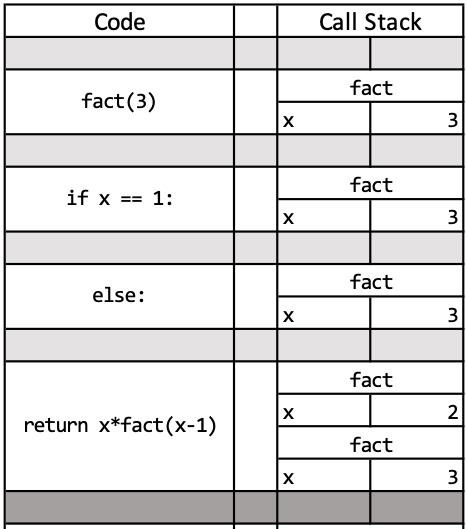
\includegraphics[width=5.9cm,height=\textheight]{images/rec-call-1.png}

}

\end{figure}
\end{frame}

\begin{frame}{Recursion and the Call Stack}
\protect\hypertarget{recursion-and-the-call-stack-1}{}
\begin{figure}

{\centering 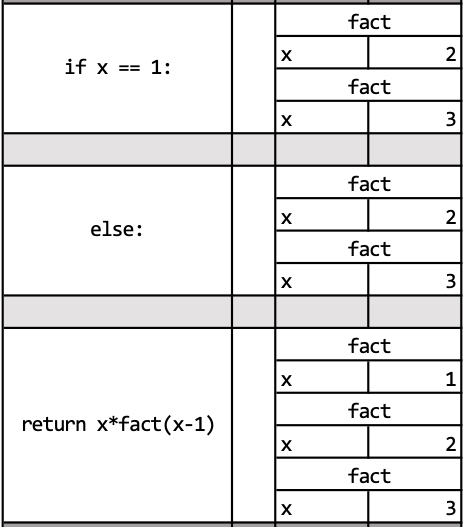
\includegraphics[width=5.9cm,height=\textheight]{images/rec-call-2.png}

}

\end{figure}
\end{frame}

\begin{frame}{Recursion and the Call Stack}
\protect\hypertarget{recursion-and-the-call-stack-2}{}
\begin{figure}

{\centering 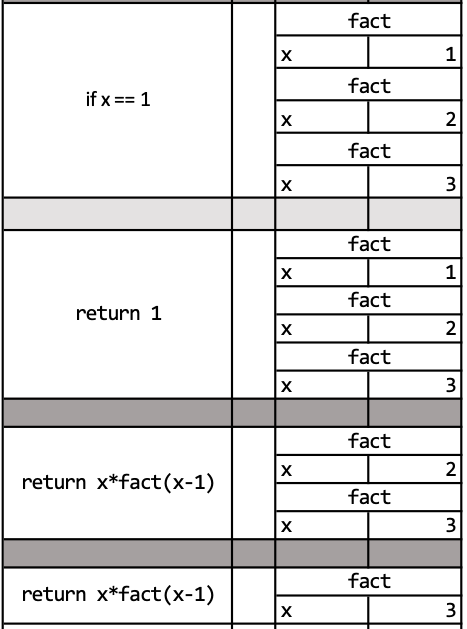
\includegraphics[width=5.9cm,height=\textheight]{images/rec-call-3.png}

}

\end{figure}
\end{frame}

\begin{frame}[fragile]{Multiple Recursive Calls: Fibonacci Sequence}
\protect\hypertarget{multiple-recursive-calls-fibonacci-sequence}{}
\begin{itemize}
\item
  In calculating the factorial, each recursion only calls itself once.
  This doesn't have to be the case
\item
  The Fibonacci Sequence is a sequence of numbers where the first two
  numbers are 0 and 1, with each subsequent number being being the sum
  of the previous two numbers in the sequence.

  \begin{itemize}
  \tightlist
  \item
    Notice how the problem is defined recursively
  \end{itemize}
\end{itemize}

\begin{Shaded}
\begin{Highlighting}[]
\KeywordTok{def}\NormalTok{ fib(n):}
  \ControlFlowTok{if}\NormalTok{ n }\OperatorTok{\textless{}=} \DecValTok{1}\NormalTok{:}
    \ControlFlowTok{return}\NormalTok{ n}
  \ControlFlowTok{else}\NormalTok{:}
    \ControlFlowTok{return}\NormalTok{ fib(n }\OperatorTok{{-}} \DecValTok{1}\NormalTok{) }\OperatorTok{+}\NormalTok{ fib(n }\OperatorTok{{-}} \DecValTok{2}\NormalTok{)}
\end{Highlighting}
\end{Shaded}

2 minutes: what is its time and space complexity?
\end{frame}

\hypertarget{time-and-space-complexity-of-recursion}{%
\section{Time and Space Complexity of
Recursion}\label{time-and-space-complexity-of-recursion}}

\begin{frame}[fragile]{Time Complexity of Recursion}
\protect\hypertarget{time-complexity-of-recursion}{}
\begin{itemize}
\item
  Generally, recursion doesn't have performance benefits compared to
  loops (in problems like finding a key in nested boxes)

  \begin{itemize}
  \tightlist
  \item
    However, it is simpler to understand
  \end{itemize}
\item
  The time complexity of recursion depends on the number of time the
  function calls itself (branches)

  \begin{itemize}
  \item
    Factorial: the \texttt{fact} is called \(n\) times before reaching
    the base case so its \(O(1^n) = O(n)\)
  \item
    If a recursive function called itself twice, then its \((2^n)\)
  \end{itemize}
\item
  When a recursive function makes multiple calls, the run time will
  often be \(O(branches^{depth})\)
\end{itemize}
\end{frame}

\begin{frame}[fragile]{Tricky Example}
\protect\hypertarget{tricky-example}{}
\begin{Shaded}
\begin{Highlighting}[]
\KeywordTok{def}\NormalTok{ recursive(n):}
  \ControlFlowTok{for}\NormalTok{ i }\KeywordTok{in} \BuiltInTok{range}\NormalTok{(n):}
    \CommentTok{\# Something happens}
\NormalTok{    i }\OperatorTok{+=} \DecValTok{2}
  \ControlFlowTok{if}\NormalTok{ n }\OperatorTok{\textless{}=} \DecValTok{0}\NormalTok{:}
    \ControlFlowTok{return} \DecValTok{1}
  \ControlFlowTok{else}\NormalTok{:}
    \ControlFlowTok{return} \DecValTok{1} \OperatorTok{+}\NormalTok{ recursive(n }\OperatorTok{{-}} \DecValTok{3}\NormalTok{)}
\end{Highlighting}
\end{Shaded}

\begin{itemize}
\item
  Loop takes \(n/2\) steps, because we increase \texttt{i} by 2
\item
  Recursion takes \(n/3\) steps \textbf{and} the loop is called
  recursively.

  \begin{itemize}
  \tightlist
  \item
    In other words, for each recursion, run the loop.
  \end{itemize}
\item
  The time complexity is \(n/2 \times n/3 = \frac{n^2}{6} = O(n^2)\)
\end{itemize}
\end{frame}

\begin{frame}{Space complexity of recursion}
\protect\hypertarget{space-complexity-of-recursion}{}
\begin{itemize}
\item
  Notice the call stack takes up space in memory. How much depends on
  the depth of the recursion
\item
  Think about the maximum amount of space the call stack will need

  \begin{itemize}
  \tightlist
  \item
    Factorial: \(O(n)\), when recursion reaches the base case
  \end{itemize}
\item
  Even when you have multiple branches, it's possible only 1 branch at
  depth \(n\) is in memory at a time
\item
  2 minutes: to find the key in nested boxes, what is the memory
  complexity of the recursive approach versus the loop approach?
\end{itemize}
\end{frame}

\hypertarget{mergesort}{%
\section{Mergesort}\label{mergesort}}

\begin{frame}{Divide and Conquer Algorithms}
\protect\hypertarget{divide-and-conquer-algorithms}{}
\begin{itemize}
\item
  Divide and Conquer (D\&C) is a general method to solve problems
  utilizing recursion.

  \begin{itemize}
  \item
    Figure out the simplest case and use it as the base case
  \item
    Figure out how to reduce your problem to the base case
  \end{itemize}
\item
  Let's start with a trivial example: how would you sum a list of
  integers?

  \begin{itemize}
  \item
    Solution is obvious with a loop
  \item
    Let's do it recursively
  \end{itemize}
\end{itemize}
\end{frame}

\begin{frame}[fragile]{Divide and Conquer Algorithms}
\protect\hypertarget{divide-and-conquer-algorithms-1}{}
Step 1

\begin{itemize}
\item
  What is the simplest array to sum?
\item
  Arrays with no elements or 1 element

  \begin{itemize}
  \tightlist
  \item
    sum of \texttt{{[}{]}} is 0, sum of \texttt{{[}8{]}} is 8
  \end{itemize}
\end{itemize}

Step 2

\begin{itemize}
\item
  How can we reduce all arrays to empty array?
\item
  Notice \texttt{sum{[}2,\ 4,\ 5{]}} = 2 + \texttt{sum{[}4,\ 5{]}}, but
  the second version reduced the problem
\end{itemize}
\end{frame}

\begin{frame}[fragile]{Divide and Conquer Algorithms}
\protect\hypertarget{divide-and-conquer-algorithms-2}{}
\begin{Shaded}
\begin{Highlighting}[]
\KeywordTok{def}\NormalTok{ rec\_sum(lst):}
  \ControlFlowTok{if} \KeywordTok{not}\NormalTok{ lst:}
    \ControlFlowTok{return} \DecValTok{0}
  \ControlFlowTok{else}\NormalTok{:}
    \ControlFlowTok{return}\NormalTok{ lst[}\DecValTok{0}\NormalTok{] }\OperatorTok{+}\NormalTok{ rec\_sum(lst[}\DecValTok{1}\NormalTok{:])}
\end{Highlighting}
\end{Shaded}

\begin{itemize}
\tightlist
\item
  Let's work on a real problem next!
\end{itemize}
\end{frame}

\begin{frame}{Mergesort}
\protect\hypertarget{mergesort-1}{}
\begin{columns}[T]
\begin{column}{0.5\textwidth}
\begin{itemize}
\item
  Some lists don't need to be sorted

  \begin{itemize}
  \tightlist
  \item
    Lists of size 1! This is our base case
  \end{itemize}
\item
  We can split lists in half until they contain 1 element, then merge
  all of the sub-lists
\item
  Python's sort function uses a hybrid of merge and insertion sort, both
  of which you've learned!
\end{itemize}
\end{column}

\begin{column}{0.5\textwidth}
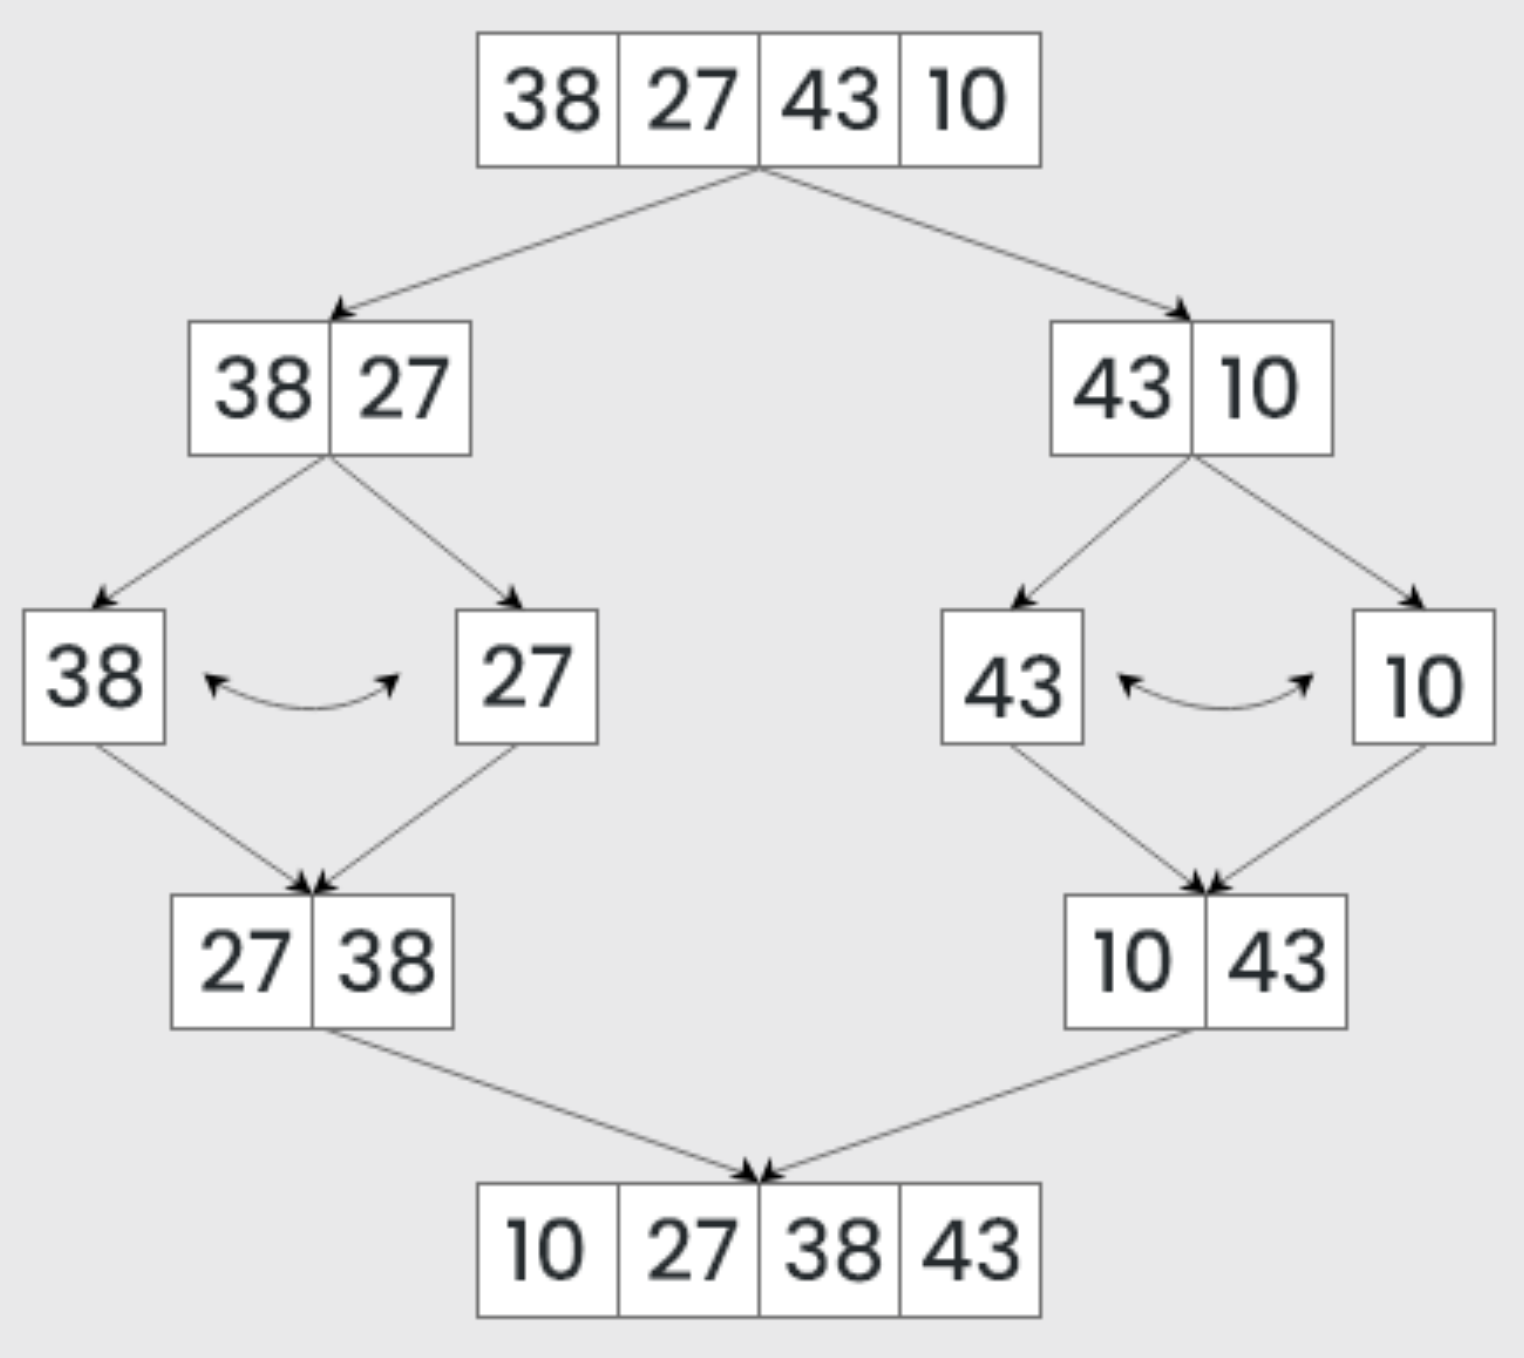
\includegraphics{images/merge-sort.png}
\end{column}
\end{columns}
\end{frame}

\begin{frame}{Big-O of Merge Sort}
\protect\hypertarget{big-o-of-merge-sort}{}
First consider the non-recursive part of the code

\begin{itemize}
\item
  The ``divide'' step takes linear time, since slicing operations take
  roughly \(n/2\) steps to make a left and right copy respectively.
\item
  The merge operation also takes \(n\) steps approximately
\item
  All other operations are constants
\item
  Together, the non-recursive part of this algorithm is \(O(n)\)
\end{itemize}

Next consider the recursive calls

\begin{itemize}
\item
  Recall the big-O of recursion depends on the recursion depth and
  number of calls. \(O(branches^{depth})\)
\item
  The depth in Merge Sort is the number of times you need to divide to
  get to a list of length 1.
\item
  Mathematically, \(2^{\text{depth}} = n\), then
  \(\text{depth} = \text{log}n\). So there are approximately log \(n\)
  levels
\end{itemize}
\end{frame}

\begin{frame}{Big-O of Mergesort}
\protect\hypertarget{big-o-of-mergesort}{}
\begin{itemize}
\item
  Since the \(O(n)\) steps must be performed each recursion, the total
  run time is \(O(n\text{log}n)\). Our analysis only depended on the
  size of the list, so the best and worst case of mergesort is the same
\item
  This is much faster than insertion sort!
\item
  2 minutes: does it have less space complexity than insertion sort?
\end{itemize}
\end{frame}

\hypertarget{recommended-problems-and-references}{%
\section{Recommended Problems and
References}\label{recommended-problems-and-references}}

\begin{frame}[fragile]{Recommended Problems}
\protect\hypertarget{recommended-problems}{}
\begin{itemize}
\item
  Bhargava: Chapter 4 exercises

  \begin{itemize}
  \tightlist
  \item
    4.1 to 4.8
  \end{itemize}
\item
  Write a recursive function that produces the
  \texttt{RecursionError:\ maximum\ recursion\ depth\ exceeded} error.
\item
  Write a iterative function to calculate the \(n\)th Fibonacci number.
  What is its time and space complexity?
\item
  Write a recursive function to determine if a string is a palindrome.
  What is its time and space complexity?
\item
  Write a recursive function to check if a given positive integer is a
  prime number. What is its time and space complexity?
\end{itemize}
\end{frame}

\begin{frame}{Recommended Problems}
\protect\hypertarget{recommended-problems-1}{}
\begin{itemize}
\item
  Suppose you have a plot of land and want to divide the land into even
  square plots, while keeping the plots as big as possible. How would
  you do this using D\&C? See Bhargava pg. 52.
\item
  Explain why the ``merge'' step in mergesort is \(O(n)\)
\item
  Implement mergesort. You might find using helper functions useful.
\item
  Write a recursive function to perform binary search on a sorted list
\end{itemize}
\end{frame}

\begin{frame}{Bonus Readings}
\protect\hypertarget{bonus-readings}{}
\begin{itemize}
\tightlist
\item
  You may be interested in learning more about quicksort in Bhargava
  chapter 4 or
  \href{https://www.teach.cs.toronto.edu/~csc148h/winter/notes/recursive-sorting/recursive_sorting.html}{here}.
  Quicksort is another recursive sorting method
\end{itemize}
\end{frame}

\begin{frame}{References}
\protect\hypertarget{references}{}
\begin{itemize}
\item
  Bhargava, A. Y. (2016). \emph{Grokking algorithms: An illustrated
  guide for programmers and other curious people.} Manning. Chapter 3
  and 4.
\item
  Cormen, T. H. (Ed.). (2009). \emph{Introduction to algorithms} (3rd
  ed). MIT Press. Chapter 4.
\end{itemize}
\end{frame}



\end{document}
